\chapter{معماری نمونه مطالعاتی برنامه پارکینگ}

\section{زمینه برنامه‌ پارکینگ}
هدف از برنامه برقراری ارتباط کاربران با پارکنیگ‌‌های مختلف و فضا‌های خالی در هر پارکینگ است؛ کاربران در این برنامه ها باید بتوانند از مکان‌های خالی در پارکینگ‌های سطح شهر آگاه شوند و امکان رزرو مکان‌های خالی را داشته باشند.در این برنامه تعداد زیاد پارکینگ‌ها در سطح شهر و تغییرات زیاد در وضعیت پارکینگ‌ها سبب پیچیدگی مدیریت سنسور‌ها می‌شود، در حالی که این پیچیدگی نباید خود را در پایگاه کد و سایر مولفه‌های سیستم نشان دهد.به منظور تفکیک دغدغه‌ها، معماری پیشنهادی برای این برنامه معماری لایه‌ای است.

در معماری لایه‌ای، لایه ها مستقل هستند بنابرین گروهی از تغییرات در یک لایه بر لایه های دیگر تأثیر نمی گذارد. با توجه به این ویژگی هر گونه تغییر در ساختار هر لایه این امکان را به ما می‌دهد تا مستقل از سایر لایه‌‌ها به بررسی تغییرات انجام شده بپردازیم. به عنوان مثال تغییر در پروتکل مورد استفاده در سنسور ها در معماری لایه‌ای صدمه ای به ساختار لایه‌های بالاتر نمی‌زند.
\section{معماری پیشنهادی}
با توجه به زمینه مطرح شده برای برنامه پارکینگ‌های شهری، معماری لایه ای پیشنهادی باید دارای لایه‌های شکل \ref{fig:parking_layer} باشد. این شکل با توجه به مقاله \cite{ahmed2019blockchain}
کشیده شده است.
\begin{figure}[h]
\centering
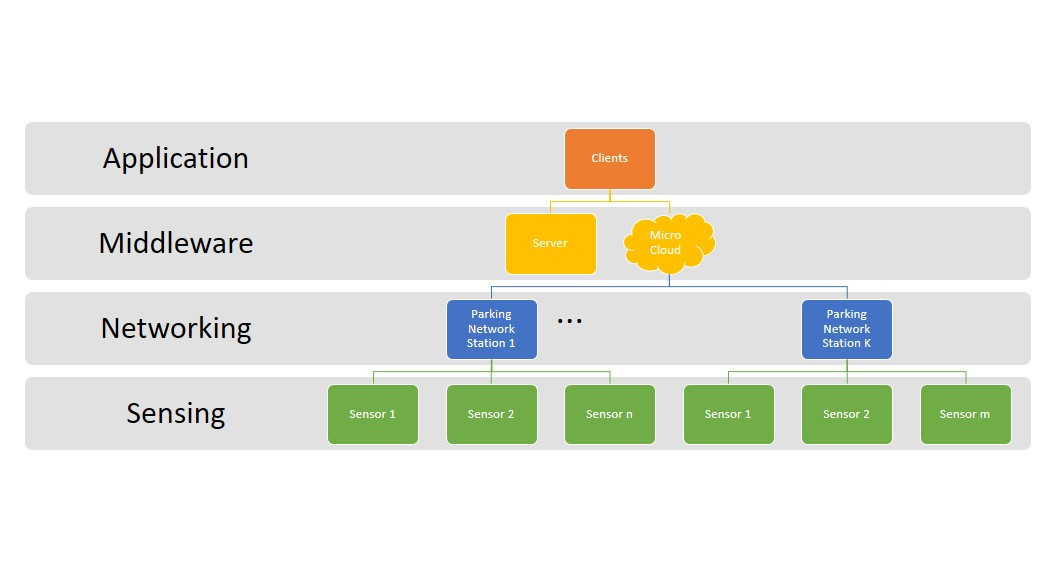
\includegraphics[scale=0.6]{parking_layer.jpg}
\caption{معماری لایه‌ای پیشنهادی برای برنامه پارکینگ‌های شهری}
\label{fig:parking_layer}
\end{figure}
در معماری لایه‌ای پیشنهادی شده حیطه عملکردی هر لایه به شرح زیر است:
\begin{itemize}
\item
لایه‌ی برنامه\LTRfootnote{Application} : برنامه‌های سمت کاربر شامل برنامه‌ی تلفن همراه و نسخه‌های وب در این لایه پیاده سازی می‌شوند و از طریق رابط ها از لایه‌ی پایینی خود خدمات را دریافت می‌کنند.کاربران قادر به جستجو در مکان های مورد نظر خود برای پارکینگ هستند و می توانند فضای مورد نظر خود را رزرو کنند.
\item
لایه میان‌افزار\LTRfootnote{Middleware} : در این لایه اطلاعات پارکینگ ها به صورت لحظه‌ای دریافت می‌شود و پس از پردازش خدماتی که کاربران در لایه‌ی برنامه نیاز دارند، در اختیارشان قرار داده می‌شود. خود سرور در این لایه از معماری میکرو سرویس تبعیت می‌کند که پیشتر ویژگی‌های آن مطرح شد.
\item
لایه شبکه \LTRfootnote{Networking} : لایه‌ی شبکه به منظور ارتباط آسان تر سنسور‌ها با لایه‌ی میان افزار تعبیه شده است. اگر قرار بود هر یک از سنسور‌ها خود مستقلا به لایه‌ی میان‌افزار وصل شوند پیچیدگی شبکه و مدیریت آن بسیار دشوار بود.لایه‌ی شبکه با تجمیع اطلاعات سنسور‌ها ضمن کشف خرابی یا اطلاعات ناصحیح در میان سنسور‌ها با پروتکل‌های مطمئن تری ضمن هزینه کمتر اطلاعات را در اختیار لایه میان‌افزار قرار می‌دهد.

لایه شبکه ارتباط بی نقص بین مراکز مختلف پارکینگ و سیستم میان‌افزار و در نهایت کاربران را تضمین می کند. داده های کاربر و مرکز پارک از طریق این لایه به سیستم میان‌افزار منتقل می شود. این لایه شامل انواع مختلف فن آوری های ارتباطی نظیر شبکه LAN و WAN است.
\item
لایه سنسور‌ها\LTRfootnote{Sensing} : سنسور‌ها از نوع های مختلف در این لایه قرار دارند و این لایه با محدود‌سازی پیچیدگی‌های سخت‌افزاری، مانع از انتشار آن به لایه‌های بالاتر خواهد شد.
\end{itemize}
\section{نیازمندی‌های پوشش‌داده شده توسط معماری}

در معماری لایه‌ای از انجا که هر لایه مستقل از دیگری است موجب اصلاح ‌پذیری بالا و قابلیت آزمون در این سیستم می‌شود. چرا که می‌توان برای مثال  در لایه سنسور‌ها، پروتکل آن‌ها و دیگر موارد را تغییر داد یا هر لایه را مجزا آزمون کرد.
همچنین در این معماری می‌توان امنیت را بر بر روی ارتباطات بین کاربران تا سرور، یا سنسورها تا میکروکلاد به راحتی داشت. 

از انجا که خود سرور از معماری میکرو کرنل استفاده می‌کند نیز خصوصیات معماری میکروکرنل نیز به آن نیز اضافه می‌شود. 

به راحتی می‌توان نیازمندی‌های مختلف را با API ها برآورده کرد که به پوشش نیازمندی‌های احراز هویت و پیاده‌سازی قابلیت استفاده پاسخ می‌دهد. آزمون راحت سرویس‌ها و تغییر آن‌ها نیز به دلیل ویژگی‌  
 \lr{loosely coupled} 
مولفه‌ها نیز امکان‌پذیر است. 

همچنین بدیل ذات توزیع شده معماری میکرو کرنل و مستقل بودن معماری لایه گسترش‌پذیری نیز امکان پذیر است که از نتایج این گسترش پذیری می‌توان به افزایش کارایی و دردسترس‌پذیری این سرویس نیز اشاره داشت.
وجود امکان ارتباط راحت با سرویس‌های دیگر نیز به قابلیت همکاری در این معماری نیز کمک می‌کند.

\section{نتیجه‌گیری}
معماری لایه‌ای با ایده‌گیری از آن چه در زیرساخت اینترنت در سراسر جهان وجود دارد یک پیشنهاد بسیار مناسب برای سیستم پارکینگ است که از یک سو با سخت افزار‌های خاص و لایه‌ی فیزیکی مشابه آن چه در شبکه اینترنت شاهد هستیم مواجه است و سمت دیگر در لایه‌ی برنامه ممکن است تغییرات بر خلاف لایه‌های پایین‌تر با سرعت بیشتری روی دهند.در لایه برنامه می‌توان الگو‌های خاصی جهت همکاری با لایه‌های پایین در استفاده کرد و معماری لایه‌ای دست معماری را برای ابتکار عمل در هر لایه باز خواهد گذاشت.
استفاده از معماری لایه ای ممکن است تغییرات در سطح وسیع به صورتی که چندین لایه را درگیر کنید را دشوارد کند و همچنین لایه ها ممکن است عملکرد برنامه را تحت تأثیر قرار دهند زیرا باعث ایجاد سربار در اجرا می شوند؛ هر لایه در سطوح بالا برای هر عملکرد در سیستم باید به لایه های پایین تر متصل شود.